\documentclass{scrreprt}
\usepackage{listings}
\usepackage{underscore}
\usepackage{graphicx}
\usepackage{xcolor}
\usepackage{tikz}
\usetikzlibrary{arrows.meta,positioning}
\usepackage[bookmarks=true]{hyperref}
\usepackage[utf8]{inputenc}
\usepackage[english]{babel}
\definecolor{tietred}{HTML}{A6192E}
\hypersetup{
    bookmarks=false,
    pdftitle={Software Requirement Specification - TiTalks},
    pdfauthor={Bhavya Agarwal, Pratham Ranka, Hitesh Arora, Ananya Yadav},
    pdfsubject={Software Engineering},
    pdfkeywords={SRS, TiTalks, React, TypeScript},
    colorlinks=true,
    linkcolor=blue,
    citecolor=black,
    filecolor=black,
    urlcolor=purple,
    linktoc=page
}%
\def\myversion{1.0 }
\date{}
\begin{document}

\begin{flushright}
    \rule{16cm}{5pt}\vskip1cm
    \begin{bfseries}
        \Huge{SOFTWARE REQUIREMENTS\\ SPECIFICATION}\\
        \vspace{1.5cm}
        for\\
        \vspace{1.5cm}
        TITALKS\\
        \vspace{1.5cm}
        \LARGE{Version \myversion}\\
        \vspace{1.5cm}
        Prepared by :\\
        1. Bhavya Agarwal (1024030304)\\
        2. Pratham Ranka (1024030301)\\
        3. Hitesh Arora (1024030298)\\
        4. Ananya Yadav (1024030299)\\
        \vspace{1.5cm}
        Submitted to : Ms. Anuskha \\
        \vspace{1.0cm}
        \today\\
    \end{bfseries}
\end{flushright}

\tableofcontents

\chapter{Introduction}

\section{Purpose}
Students of Thapar Institute of Engineering and Technology (TIET) currently depend on several unrelated channels to discover campus events, follow societies, find peers and exchange updates. Information is fragmented, important announcements compete with general-purpose content, and a user's identity is not necessarily tied to the institute. "TiTalks" addresses this gap. It is a campus-centred social networking application that gives TIET students one focused space for announcements, societies, events, collaboration and peer interaction, in a familiar visual social experience restricted conceptually to the TIET community.
\newline
This document specifies the requirements of TiTalks. The current deliverable is a feature-rich client-side prototype (React screens, typed mock data, local state, browser storage and local media). A real server, database, Google OAuth, permanent media storage and realtime communication are reserved for the next development phase, and are specified here as planned requirements.

\section{Intended Audience and Reading Suggestions}
This SRS is for developers, project managers, users, faculty evaluators and testers. The discussion provides the functional and non-functional information about "TiTalks". Developers and testers should read all chapters; evaluators may focus on Chapters 1 to 3.

\section{Project Scope}
"TiTalks" creates a space for TIET students and club or society users to connect, share and discover campus activity.
\newline
A user signs in with an institutional email under the \texttt{thapar.edu} domain (or its subdomains); personal or misleading domains are rejected by the prototype. After registration, the user completes profile onboarding and enters the application.
\newline
Users can browse a feed of posts, view and create stories, watch reels, search for people, explore campus events on the Pulse page, exchange direct and group messages, and view notifications and follow requests.
\newline
Users can like, save, comment, share, follow, create, edit, archive, restore and delete content, and can report, block or mute content and accounts. In the prototype these actions change local interface state only.
\newline
Profiles contain post, saved and tagged grids, follower and following lists, highlights, archived posts, and privacy, notification and appearance settings.
\newline
\begin{figure}[h!]
\centering
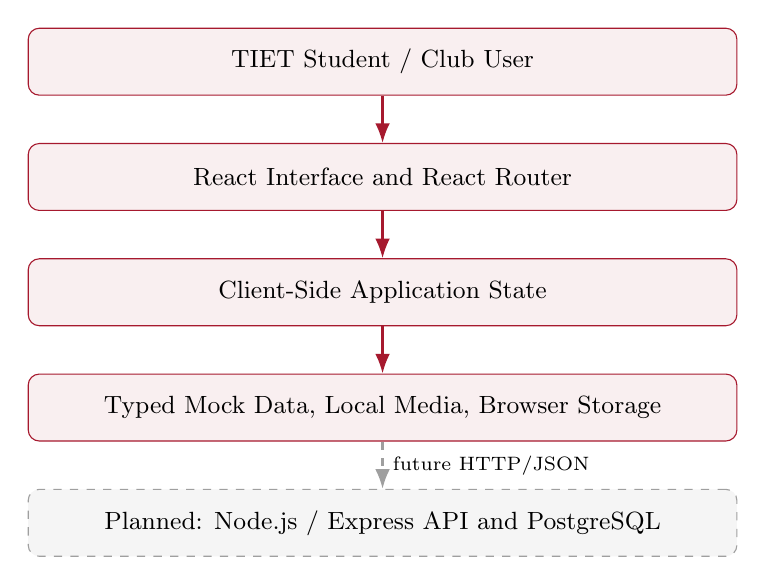
\begin{tikzpicture}[
  node distance=0.6cm,
  box/.style={draw=tietred, rounded corners, fill=tietred!7, minimum width=9cm, minimum height=0.85cm, align=center, font=\small},
  pbox/.style={draw=gray!75, rounded corners, fill=gray!8, dashed, minimum width=9cm, minimum height=0.85cm, align=center, font=\small},
  cur/.style={-{Latex[length=2.5mm]}, thick, draw=tietred},
  pln/.style={-{Latex[length=2.5mm]}, thick, dashed, draw=gray!75}
]
  \node[box] (user) {TIET Student / Club User};
  \node[box, below=of user] (ui) {React Interface and React Router};
  \node[box, below=of ui] (state) {Client-Side Application State};
  \node[box, below=of state] (local) {Typed Mock Data, Local Media, Browser Storage};
  \node[pbox, below=of local] (be) {Planned: Node.js / Express API and PostgreSQL};
  \draw[cur] (user) -- (ui);
  \draw[cur] (ui) -- (state);
  \draw[cur] (state) -- (local);
  \draw[pln] (local) -- node[right, font=\scriptsize]{future HTTP/JSON} (be);
\end{tikzpicture}
\caption{Entire work-flow and architecture (solid: implemented, dashed: planned)}
\label{fig:workflow}
\end{figure}
\newline
Figure~\ref{fig:workflow} is the overview of the project. The user interacts with React screens, the screens update client-side state, and that state reads and writes mock data and browser storage. In the next phase the frontend will talk to the planned API and database.

\chapter{Overall Description}

\section{Product Perspective}
"TiTalks" replaces the scattered use of general social media, chat groups and notice boards for campus communication with a single institute-focused application. The product follows a prototype-first approach: the full user experience is built and validated on the client before backend infrastructure is added. The main goal is to validate the product flow and to keep the interface reusable when mock data is later replaced by real APIs.

\section{User Classes and Characteristics}
"TiTalks" has basically 2 types of users.
\begin{itemize}
  \item Student (TIET student with a \texttt{thapar.edu} account)
  \item Club / Society user
\end{itemize}
Students complete sign-in and onboarding and then use the feed, discovery, messaging and profile features. Club or society users access the same screens and actions as students; societies appear as part of the campus-relevant sample content. Server-side moderation roles are not part of the current prototype and are left to the planned backend phase.
\begin{figure}[h!]
\centering
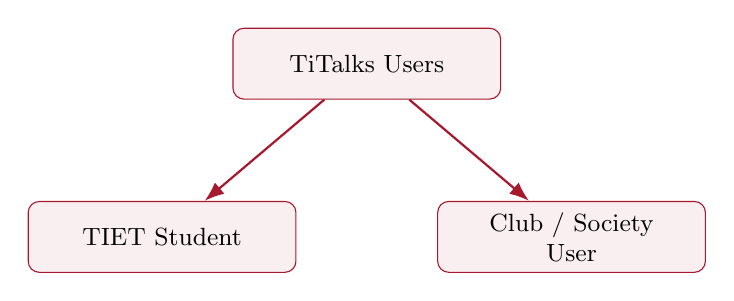
\begin{tikzpicture}[
  box/.style={draw=tietred, rounded corners, fill=tietred!7, minimum width=3.4cm, minimum height=0.9cm, align=center, font=\small},
  ln/.style={-{Latex[length=2.5mm]}, thick, draw=tietred}
]
  \node[box] (root) at (0,0) {TiTalks Users};
  \node[box] (stu) at (-2.6,-2.2) {TIET Student};
  \node[box] (club) at (2.6,-2.2) {Club / Society\\User};
  \draw[ln] (root) -- (stu);
  \draw[ln] (root) -- (club);
\end{tikzpicture}
\caption{Type of users}
\label{fig:usertypes}
\end{figure}

\section{Product Functions}
"TiTalks" provides the following functions: authentication and onboarding; feed, posts, stories and reels; discovery of people and events; messaging; notifications; profile and settings management; and safety controls.
\newline
Users have - profile information, privacy settings, notification settings and a theme preference.
\newline
Posts have - author information, location, caption, tags, media and engagement counts.
\newline
Stories and reels have - author, media (image or video), highlight selection and archive state.
\newline
Events have - a category, event details and an add-to-my-day action.
\newline
Conversations are direct or group and contain text and image messages.
\newline
Notifications include activity notifications and follow requests.
\newline
Figure~\ref{fig:dfd} shows how these functions exchange data.
\begin{figure}[h!]
\centering
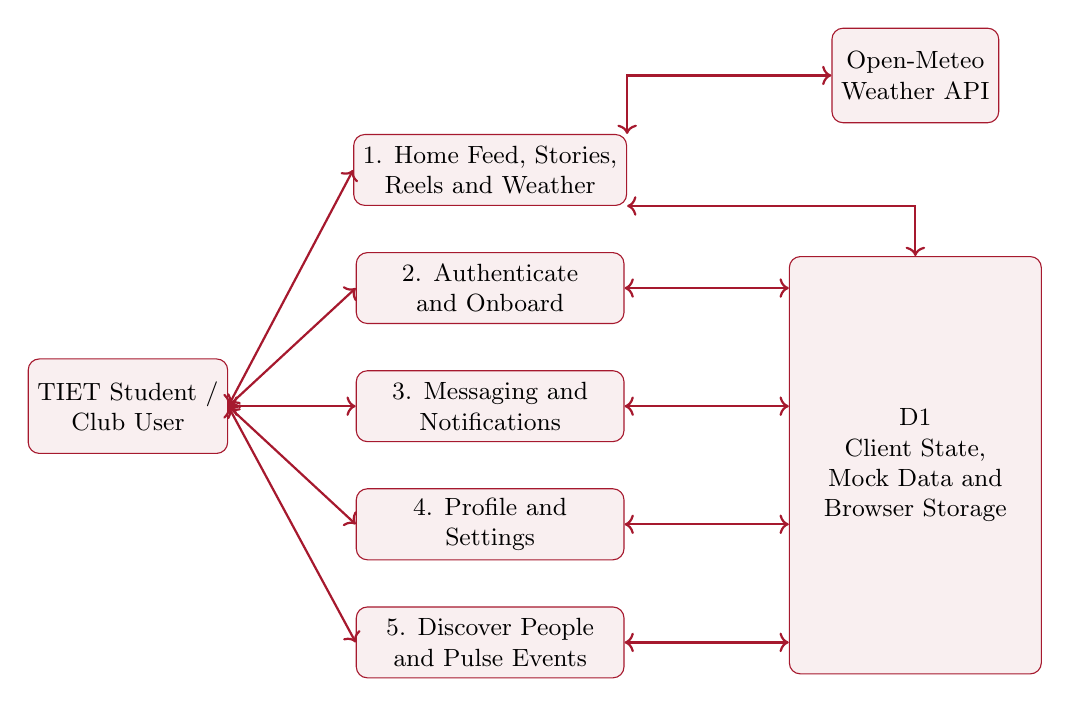
\begin{tikzpicture}[
  ent/.style={draw=tietred, rounded corners, fill=tietred!7, minimum width=2cm, minimum height=1.2cm, align=center, font=\small},
  proc/.style={draw=tietred, rounded corners, fill=tietred!7, minimum width=3.4cm, minimum height=0.9cm, align=center, font=\small},
  store/.style={draw=tietred, rounded corners, fill=tietred!7, minimum width=3.2cm, align=center, font=\small},
  fl/.style={<->, thick, draw=tietred}
]
  \node[ent] (user) at (0,0) {TIET Student /\\Club User};
  \node[proc] (p2) at (4.6,3) {1. Home Feed, Stories,\\Reels and Weather};
  \node[proc] (p1) at (4.6,1.5) {2. Authenticate\\and Onboard};
  \node[proc] (p3) at (4.6,0) {3. Messaging and\\Notifications};
  \node[proc] (p4) at (4.6,-1.5) {4. Profile and\\Settings};
  \node[proc] (p5) at (4.6,-3) {5. Discover People\\and Pulse Events};
  \node[store, minimum height=5.3cm] (ds) at (10,-0.75) {D1\\Client State,\\Mock Data and\\Browser Storage};
  \node[ent] (api) at (10,4.2) {Open-Meteo\\Weather API};
  \foreach \p in {p1,p3,p4,p5}{
    \draw[fl] (\p.east) -- (\p.east -| ds.west);
  }
  \foreach \p in {p1,p2,p3,p4,p5}{
    \draw[fl] (user.east) -- (\p.west);
  }
  \draw[fl] (p2.south east) -| (ds.north);
  \draw[fl] (p2.north east) |- (api.west);
\end{tikzpicture}
\caption{Data Flow Diagram (Level 1) of the current prototype}
\label{fig:dfd}
\end{figure}

\section{Operating Environment}
The application is a single-page web application that runs in a modern web browser on desktop and mobile devices. It has been verified with headless Chromium on desktop and mobile viewports. The interface adapts between desktop (expandable sidebar and collapsible agenda rail) and mobile (bottom navigation). The live weather widget requires internet access; all other demo content is bundled locally.

\section{Design}
Student activities have 4 steps -
\begin{itemize}
    \item Sign in with institutional email
    \item Profile onboarding
    \item Browse feed, stories, reels and events
    \item Create content, message and manage profile
\end{itemize}
A student first signs in with a \texttt{thapar.edu} email. After validation and onboarding, the student enters the home feed. Every profile contains personal information, posts, saved items, tagged items, highlights, archived posts and follower lists.
\begin{figure}[h!]
\centering
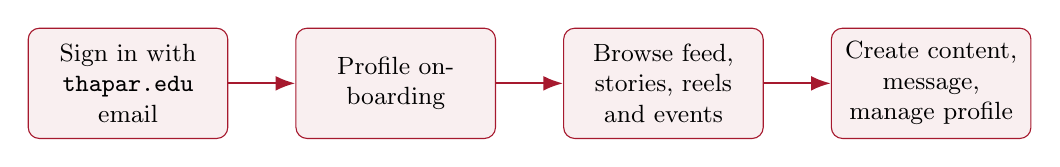
\begin{tikzpicture}[
  box/.style={draw=tietred, rounded corners, fill=tietred!7, text width=2.3cm, minimum height=1.4cm, align=center, font=\small},
  ln/.style={-{Latex[length=2.5mm]}, thick, draw=tietred}
]
  \node[box] (a) at (0,0) {Sign in with \texttt{thapar.edu} email};
  \node[box] (b) at (3.4,0) {Profile onboarding};
  \node[box] (c) at (6.8,0) {Browse feed, stories, reels and events};
  \node[box] (d) at (10.2,0) {Create content, message, manage profile};
  \draw[ln] (a) -- (b);
  \draw[ln] (b) -- (c);
  \draw[ln] (c) -- (d);
\end{tikzpicture}
\caption{Student activities}
\label{fig:studentact}
\end{figure}
\newline
Club or society users perform the same activities as students.
\newline
Content owners can manage their content through the following activities -
\begin{itemize}
    \item Create, edit, archive, restore and delete posts, stories and reels
\end{itemize}
\begin{figure}[h!]
\centering
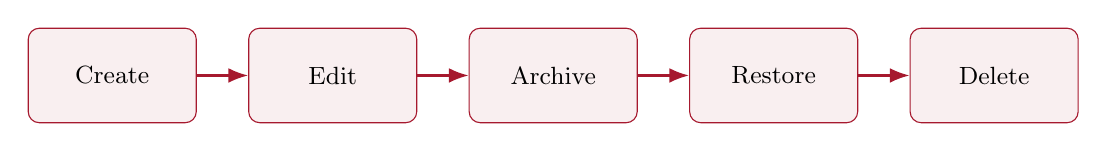
\begin{tikzpicture}[
  box/.style={draw=tietred, rounded corners, fill=tietred!7, text width=1.9cm, minimum height=1.2cm, align=center, font=\small},
  ln/.style={-{Latex[length=2.5mm]}, thick, draw=tietred}
]
  \node[box] (a) at (0,0) {Create};
  \node[box] (b) at (2.8,0) {Edit};
  \node[box] (c) at (5.6,0) {Archive};
  \node[box] (d) at (8.4,0) {Restore};
  \node[box] (e) at (11.2,0) {Delete};
  \draw[ln] (a) -- (b);
  \draw[ln] (b) -- (c);
  \draw[ln] (c) -- (d);
  \draw[ln] (d) -- (e);
\end{tikzpicture}
\caption{Content management activities}
\label{fig:contentact}
\end{figure}
\newline
Safety activities (report, block, mute and unfollow) currently change local interface state only; enforcement across accounts is planned for the backend phase.
\begin{figure}[h!]
\centering
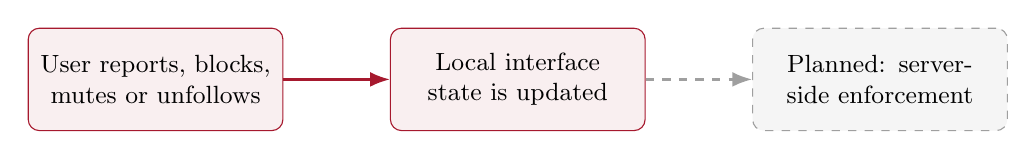
\begin{tikzpicture}[
  box/.style={draw=tietred, rounded corners, fill=tietred!7, text width=3cm, minimum height=1.3cm, align=center, font=\small},
  pbox/.style={draw=gray!75, rounded corners, fill=gray!8, dashed, text width=3cm, minimum height=1.3cm, align=center, font=\small},
  ln/.style={-{Latex[length=2.5mm]}, thick, draw=tietred},
  pln/.style={-{Latex[length=2.5mm]}, thick, dashed, draw=gray!75}
]
  \node[box] (r) at (0,0) {User reports, blocks, mutes or unfollows};
  \node[box] (v) at (4.6,0) {Local interface state is updated};
  \node[pbox] (x) at (9.2,0) {Planned: server-side enforcement};
  \draw[ln] (r) -- (v);
  \draw[pln] (v) -- (x);
\end{tikzpicture}
\caption{Safety activities (solid: implemented, dashed: planned)}
\label{fig:safetyact}
\end{figure}
The presentation layer renders React views, the navigation layer maps URLs via React Router, the client state layer stores temporary posts, reactions, follows and archive state with browser local storage preserving the session, profile settings and theme, and the data layer provides typed mock records and bundled WebP/MP4 assets.

\chapter{System Features}
"TiTalks" is a campus social networking web application. Its core value is authenticated, institute-focused sharing and discovery of campus content.

\section{Description and Priority}
"TiTalks" has main features and supporting features, and all of them are needed for a complete campus experience.
\newline
The features in order of priority -
\begin{enumerate}
    \item Authentication and Onboarding : This is the entry point. It validates \texttt{thapar.edu} emails, supports mock Google account selection, registration, password recovery navigation and profile onboarding.
    \item Feed, Posts and Stories : Central feed with author, location, caption, tags, media and engagement counts. Users like, save, share and comment, and can create posts and stories. Story navigation supports the keyboard.
    \item Reels : Local video playback, interaction controls, creation, editing, deletion and incremental loading.
    \item Discovery (People and Pulse) : Search of people, follow actions, event category filtering, event details, add-to-my-day and a responsive TIET campus map viewer. The home page includes a live Patiala weather widget.
    \item Messaging : Direct and group conversations, text and image messages and automatic scrolling to recent messages.
    \item Notifications : Activity view for notifications and follow requests.
    \item Profile and Settings : Post, saved and tagged grids, follower and following lists, highlights, archive, profile editing, privacy and notification controls, theme, logout and account-deletion UI.
    \item Safety Controls : Edit, archive, restore, delete, report, block, mute and unfollow flows.
\end{enumerate}

\section{Functional Requirements}
The "TiTalks" prototype is built with React 18, TypeScript, Vite, Tailwind CSS v4, React Router, Lucide React and Lenis.
\newline
Front-End - React 18, TypeScript, Vite, Tailwind CSS v4, React Router.
\newline
Data (current) - typed mock data, bundled media, browser local storage; weather from the Open-Meteo API.
\newline
Back-End (planned) - Node.js, Express, Google OAuth, durable media storage.
\newline
Database (planned) - PostgreSQL.
\newline
Testing - Vitest, Testing Library, jsdom, Playwright Core and custom Node.js deployment checks.
\newline
The functional requirements are listed below.
\begin{enumerate}
    \item FR1: The system shall accept sign-in and registration only for emails under \texttt{thapar.edu} or its subdomains, after normalizing case, and shall reject personal, malformed and empty emails.
    \item FR2: The system shall validate password length and required profile fields before completing sign-in or onboarding.
    \item FR3: The system shall keep the current session in a versioned local-storage key so the demo survives a page refresh.
    \item FR4: The system shall let users like, save, comment on and share posts, and open routed post details.
    \item FR5: The system shall let users create posts, stories and reels with local media, and edit, archive, restore and delete their own content.
    \item FR6: The system shall let users manage stories, including replacement, deletion and highlight selection.
    \item FR7: The system shall play local reels with interaction controls and incremental loading.
    \item FR8: The system shall let users search people, follow and unfollow, and open other-user profile routes.
    \item FR9: The system shall let users filter events by category, view event details, add an event to their day and view the campus map.
    \item FR10: The system shall show live Patiala weather with explicit loading, success and error states.
    \item FR11: The system shall support direct and group conversations with text and image messages.
    \item FR12: The system shall show notifications and follow requests.
    \item FR13: The system shall let users report, block and mute content or accounts and unfollow users.
    \item FR14: The system shall let users edit profile, privacy, notification and theme settings, and shall persist the selected light or dark theme.
    \item FR15: The system shall provide direct URL routing for all major screens, with a not-found view.
    \item FR16 (planned): The system shall authenticate through Google OAuth restricted to TIET accounts with server-side sessions.
    \item FR17 (planned): The system shall persist users, posts, comments, reactions, follows and messages in PostgreSQL through a REST API.
    \item FR18 (planned): The system shall validate and store uploaded media durably, with ownership checks, size limits and content-type restrictions.
    \item FR19 (planned): The system shall deliver realtime messaging and notifications.
    \item FR20 (planned): The system shall enforce privacy, block, mute, report, archive and deletion rules on the server.
\end{enumerate}

\chapter{Other Nonfunctional Requirements}

\section{Performance Requirements}
"TiTalks" is used on both desktop and mobile, so the interface must stay responsive. Route-level code splitting keeps optional screens out of the initial bundle. The current production build has an entry JavaScript bundle of about 301.54~kB (91.25~kB gzip) and a stylesheet of about 71.52~kB (11.59~kB gzip). These are build sizes and a baseline for optimization, not network latency measurements. Concurrent-user performance and realtime messaging will be measured once the backend exists.

\section{Security Requirements}
In the current prototype, the sign-in flow only checks that the email belongs to \texttt{thapar.edu}; authentication is a mock and is not a secure system. Once the backend exists, the system shall allow only authenticated TIET accounts to enter the application, and each user shall be able to perform only his/her own actions, such as editing or deleting own content. Password verification, Google OAuth tokens, server sessions, rate limiting, authorization checks, upload validation, and enforceable report, block and mute rules require the planned backend. The system must not be described as production-ready until these are implemented.

\section{Software Quality Attributes}
Quality is checked continuously during development so that the requirements remain fulfilled. Accessibility: buttons use accessible labels, status feedback uses live regions, relevant dialogs close with the keyboard, and animations respect reduced-motion preferences in line with WCAG 2.2. Maintainability: typed shared models, reusable feature-based components and a clear frontend-to-backend handoff. Usability: responsive layouts with explicit loading, empty, error and not-found states.
\newline
Unit, integration, build, browser and staging tests are required. The combined command \texttt{npm run test:all} is the regression gate. The latest verified results are in Table~\ref{tab:quality}.
\begin{table}[h]
\centering
\begin{tabular}{|p{0.30\textwidth}|p{0.22\textwidth}|p{0.34\textwidth}|}
  \hline
  \textbf{Metric} & \textbf{Target} & \textbf{Achieved} \\
  \hline
  Automated test cases & All pass & 54 of 54 passed \\
  \hline
  Test files & All pass & 7 of 7 passed \\
  \hline
  Source files mapped to tests & Every file covered & 39 of 39 \\
  \hline
  TypeScript check & Zero errors & Passed \\
  \hline
  Production build & Successful bundle & Passed (1,628 modules) \\
  \hline
  Browser smoke test & Critical flows pass & Passed, desktop and mobile \\
  \hline
  Staging deep routes & Seven routes available & 7 of 7 passed \\
  \hline
  Browser page errors & Zero & Zero detected \\
  \hline
\end{tabular}
\caption{Verified quality-gate results}
\label{tab:quality}
\end{table}
The pass rate applies to the defined test cases and is not a claim of 100\% source-code coverage.

\section{Business Rules}
"TiTalks" is intended for the TIET community and focuses on campus content such as societies, events and locations. It saves students the effort of following many unrelated channels. Content owners alone may edit, archive or delete their content. Moderation decisions must be enforced server-side once the backend exists.

\chapter{Other Requirements}
"TiTalks" needs maintenance as it is a long-running product. The next milestone is not a redesign of the interface but connecting the validated flows to secure, persistent backend services: Google OAuth for TIET accounts, a Node.js/Express REST API, PostgreSQL with migrations and constraints, validated media uploads, realtime messaging and notifications, and server-side enforcement of privacy and moderation rules. The test suite must be extended with API, database, authorization, security, accessibility, load and user-acceptance tests, and continuous integration should run \texttt{npm run test:all} before every merge or deployment. Real-user performance and accessibility should be measured after deployment, and requirements may change as campus needs evolve.

\begin{thebibliography}{99}
\bibitem{react} Meta Open Source, \emph{React Documentation}, 2026.
\bibitem{typescript} Microsoft, \emph{TypeScript Documentation}, 2026.
\bibitem{vite} Vite Team, \emph{Vite Documentation}, 2026.
\bibitem{tailwind} Tailwind Labs, \emph{Tailwind CSS Documentation}, 2026.
\bibitem{playwright} Microsoft, \emph{Playwright Documentation}, 2026.
\bibitem{wcag} World Wide Web Consortium, \emph{Web Content Accessibility Guidelines (WCAG) 2.2}, 2023.
\bibitem{openmeteo} Open-Meteo, \emph{Open-Meteo Weather API Documentation}, 2026.
\end{thebibliography}

\end{document}